\twocolumn[{%
\makeatletter
\section{Interaction Trace and Test Cases}\label{app:trace}\label{app:tests}
\centering
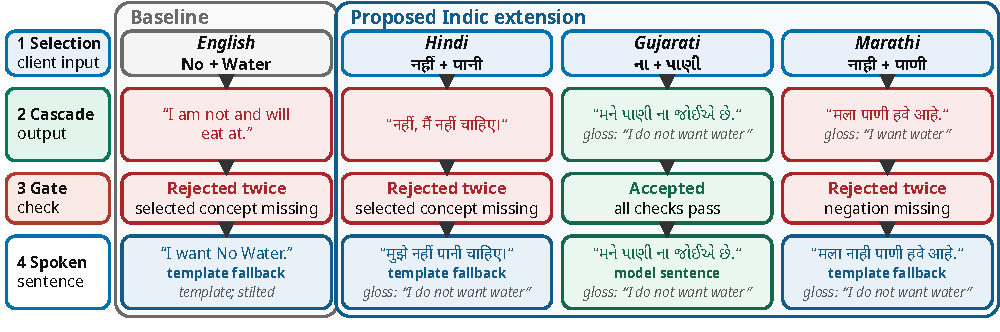
\includegraphics[width=\textwidth]{figures/fig4_languages.pdf}
\captionof{figure}{One selection (\emph{No}\,+\,\emph{Water}) in four languages (recorded outputs, client input). Red: rejected cascade output; blue: template fallback; green: accepted model sentence; italics: the authors' gloss. The word order of the template sentences is not native-reviewed.}
\label{fig:workflow}
\vspace{2pt}
\centering\footnotesize
\setlength{\tabcolsep}{3.2pt}\renewcommand{\arraystretch}{1.02}
\begin{tabular}{@{}L{2.5cm}L{2.95cm}L{2.85cm}L{3.0cm}L{3.0cm}@{}}
\toprule
\rowcolor{headtint}
Family ($n$): selection & \lang{English} (baseline) & \lang{Hindi} & \lang{Gujarati} & \lang{Marathi} \\
\midrule
Request (35): \emph{Fruit}
 & \kept{I want Fruit.} \routet\ \okmark
 & \hi{\kept{मुझे फल चाहिए।}} \routem\ \okmark
 & \gu{\kept{મને ફળ જોઈએ છે.}} \routem\ \okmark
 & \hi{\kept{मला फळ हवे आहे.}} \routem\ \okmark \\
\rowcolor{rowtint}
Refusal (38): \emph{No}\,+\,\emph{Fruit}
 & \bad{I am not a} \sel{fruit}\bad{. I do not eat fruits.} \routem\ \failmark{W,A}
 & \hi{\kept{फल नहीं है, नहीं चाहिए।}} \routem\ \okmark
 & \gu{\sel{મારે ના ફળ છે.}} \routem\ \failmark{N}
 & \hi{\kept{मला नाही फळ हवे आहे.}} \routet\ \okmark \\
Feeling (30): \emph{Angry}
 & \bad{I want} \sel{Angry.} \routet\ \failmark{W}
 & \hi{\bad{मुझे} \sel{गुस्सा} \bad{चाहिए।}} \routem\ \failmark{W}
 & \gu{\bad{મને} \sel{ગુસ્સો} \bad{જોઈએ છે.}} \routem\ \failmark{W}
 & \hi{\bad{मला} \sel{रागात} \bad{हवे आहे.}} \routem\ \failmark{W} \\
\rowcolor{rowtint}
Negated feeling (32): \emph{No}\,+\,\emph{Angry}
 & \bad{I want} \sel{No Angry.} \routet\ \failmark{W}
 & \hi{\sel{गुस्सा,} \bad{नहीं चाहिए।}} \routem\ \failmark{W}
 & \gu{\sel{મારે ના ગુસ્સો છે.}} \routem\ \failmark{N}
 & \hi{\bad{मला} \sel{नाही रागात} \bad{हवे आहे.}} \routet\ \failmark{W} \\
Action (24): \emph{Drink}\,+\,\emph{Milk}
 & \bad{The user requested} \sel{milk} \bad{for their drink.} \routem\ \failmark{N,P}
 & \hi{\kept{मुझे पीना दूध चाहिए।}} \routet\ \okmark
 & \gu{\kept{મને પીવું જોઈએ છે. દૂધ આપે.}} \routem\ \okmark
 & \hi{\kept{मला पिणे दूध हवे आहे.}} \routem\ \okmark \\
\rowcolor{rowtint}
Call (16): \emph{Call}\,+\,\emph{Doctor}
 & \kept{I want Call Doctor.} \routet\ \okmark
 & \hi{\kept{फ़ोन करना गया है, मुझे डॉक्टर चाहिए।}} \routem\ \okmark
 & \gu{\sel{મને ડૉક્ટર ફોન કરવો છે.}} \routem\ \failmark{N}
 & \hi{\sel{मला डॉक्टर फोन करणे मिळू शकता का?}} \routem\ \failmark{N} \\
\bottomrule
\end{tabular}
\captionof{table}{One scenario per family (the first alphabetical one present in all four languages), deployed output with client input (recorded). Intended messages: \gloss{I want fruit}, \gloss{I do not want fruit}, \gloss{I am angry}, \gloss{I am not angry}, \gloss{I want to drink milk}, \gloss{I want to call the doctor}. Colors, marks, and tags as in Table~\ref{tab:analysis}; \failmark{P}: third-person report. Green marks a scorer pass, not fluency (\emph{I want Call Doctor.}); no native speaker has judged these outcomes; the Gujarati and Marathi \emph{Call} outputs are a scorer gap and a question form.}
\label{tab:grid}
\makeatother
}]

\begin{table*}[!t]
\centering\footnotesize
\setlength{\tabcolsep}{3.2pt}\renewcommand{\arraystretch}{1.02}
\begin{tabular}{@{}L{2.9cm}L{2.3cm}L{5.2cm}L{5.1cm}@{}}
\toprule
\rowcolor{headtint}
Kind of outcome & Input & Recorded output & Result \\
\midrule
Unrequested content, caught & \lang{English}, client: \emph{No}\,+\,\emph{Water} & first candidate \bad{I am not hungry. I will eat at the restaurant.} & rejected: concept missing, and \emph{hungry} and \emph{restaurant} are forbidden words \\
\rowcolor{rowtint}Code-mixed input (exploratory) & \lang{Hinglish}, API input: \emph{Pizza} & \bad{The user requested a pizza.} \routem & accepted by the gate; fails scorer (third person, English for Hindi); the template baseline succeeds \\
Ambiguous selection; server unreachable (repaired client) & \lang{English}: \emph{Nose}; any language & card \gloss{What do you want to say?} with buttons \gloss{I want something} and \gloss{I feel something}; literal labels as a preview & nothing is spoken until the user chooses; nothing is guessed \\
\bottomrule
\end{tabular}
\caption{One recorded example of each further kind of outcome (colors and tags as in Table~\ref{tab:analysis}; Figure~\ref{fig:teaser} shows three more kinds). The last row shows demo states of the repaired build, not scored scenarios.}
\label{tab:kinds}
\end{table*}


\begin{table*}[!t]
\centering\footnotesize
\setlength{\tabcolsep}{3pt}\renewcommand{\arraystretch}{1.02}
\begin{tabular}{@{}L{4.0cm}L{8.1cm}L{3.4cm}@{}}
\toprule
\rowcolor{headtint}
Component and role & Training or adaptation & Data or license \\
\midrule
\qwen{}: realizer, refiner, verifier & Prompted, not fine-tuned (few-shot for HI, GU, MR); rev.\ 7ae5576 & Apache-2.0 \\
\indicf{} + \vocos{}: speech & Pretrained; zero-shot voice from a clip and its transcript & 1,417\,h; MIT, gated \\
HMM-1, HMM-2: optional next word, Un-Jumble & Streamed in 500K-sentence chunks, count-pruned; HMM-1: Jelinek--Mercer weights 0.50/0.30/0.15/0.05; HMM-2: word and part-of-speech trigrams, beam 64 & English sentences, Tatoeba, Pile slices \\
Gutenberg HMM, Hindi AAC HMM: baselines & Bigram and trigram counts over 188,402 sentences (713,845 trigram states); 3,867 Hindi turns (3,078 for evaluation) & public-domain books; Hindi dialogues \\
Suffix trie ($\infty$-gram): primary next word & Count-based, built at start-up (\IGSent{} sentences, depth \IGDepth{}) & English and Hindi dialogues \\
\flant{} refiner: companion tool & Fine-tuned (learning rate $10^{-4}$, batch 16 with two accumulation steps, 10 epochs, seed 42, one TITAN Xp, 204\,s) after a 500-update fluency adaptation on 4,380 denoising pairs; on 384 test inputs it reaches \RefAModel{} exact match (\RefFModel{} with the adaptation) and no negation error in 172 negated inputs; rules score \RefARules{} (references come from the same templates) & 3,052 template inputs (384 validation, 384 test) \\
\bottomrule
\end{tabular}
\caption{Learned components, from the training records and model files in the release package; \qwen{} and \indicf{} are used as released; Noto fonts: SIL OFL 1.1.}
\label{tab:models}
\end{table*}

\begin{table*}[!t]
\centering\footnotesize
\setlength{\tabcolsep}{3.4pt}\renewcommand{\arraystretch}{1.1}
\begin{tabular}{@{}l c ccc cccc c@{}}
\toprule
\rowcolor{headtint}
 & Evaluated build & \multicolumn{3}{c}{Human voice prompts} & \multicolumn{4}{c}{Stand-in voice, deployed sentences} & Deployed voice \\
\rowcolor{headtint}
 & \lang{Tone} (1) & \lang{English} (1) & \lang{Marathi} (3) & \lang{Punjabi} (1) & \lang{English} (46) & \lang{Hindi} (45) & \lang{Gujarati} (42) & \lang{Marathi} (42) & \indicf{} (0) \\
\midrule
\utmos{} & \bad{1.54} & 4.27 & 3.20 & 3.83 & 4.01 (0.31) & 3.66 (0.38) & 3.88 (0.24) & 3.31 (0.41) & not run \\
\rowcolor{rowtint}\nisqa{} & \bad{1.12} & 4.50 & 4.81 & 4.74 & 4.39 (0.61) & 3.52 (0.59) & 4.91 (0.10) & 3.95 (0.64) & not run \\
\bottomrule
\end{tabular}
\caption{Predicted speech quality (1--5, higher is better; mean, and standard deviation for the synthesized voices; clips in the header). \emph{Tone}: the evaluated build's placeholder. Human prompts: clips that \indicf{} would imitate (Punjabi: the default for all languages). Stand-in voices: open \mmstts{} models reading the deployed sentences, not \indicf{}, whose weights are gated. Both predictors are trained on English ratings (indicative only).}
\label{tab:mos}
\end{table*}


\section{Scorer, Failure Audit, Speech, and Runtime}
\label{app:scorer}\label{app:coverage}
Retention is the share of required concept instances present. Polarity is correct when a negator is present exactly if the gold message is negated (its scope is not checked), and the act is correct when a request marker (want, need, \hi{चाहिए}, \gu{જોઈએ}, \hi{हवे}) or, for feelings, a feeling marker without a request marker is present. A concept is \emph{added} if any other board concept or a time, meal, or venue word occurs.
An output is \emph{off-task} if it is a model refusal or meta-comment, is a third-person report (``the user\ldots''; English only), is empty or longer than 25 tokens, or contains Latin text in an Indic target; a user's own refusal is never off-task. With explicit fields, feelings carry the intent \textsc{statement} (chosen after an aborted 54-request pilot).
\emph{Failure audit.} Of the 37 accepted outputs that fail the scorer with explicit fields, 35 are genuine failures (12 negated want for a negated feeling, 10 ungrammatical, 9 third-person reports, 4 added content) and two are marker-list gaps, as are all six failing template fallbacks and all eight failing template-only outputs (AI-assisted classification, not native-checked).
Exploratory Hinglish (8 scenarios; client input, explicit fields): deployed \CMSuccDepU{}, \CMSuccDepS{}; unconstrained \CMSuccNaive{}; template baseline \CMSuccTmplU{}, \CMSuccTmplS{}.


Speech routes to \indicf{} with the default Punjabi reference clip for every language; browser voices (hi-IN, gu-IN, mr-IN, en-US; Gujarati and Marathi fall back to hi-IN, then en-IN) speak only when the server returns no audio. Neither route was verified: the gated weights were absent (placeholder tone) and the test browser exposed no voices. Table~\ref{tab:mos} scores the tone, the prompt clips, and, as a pipeline check only, the deployed sentences read by open \mmstts{} voices \citep{pratap2023mms}, with \utmos{} \citep{saeki2022utmos} and \nisqa{} \citep{mittag2021nisqa}; both are trained on English ratings, so the values are indicative and do not describe \indicf{}.
Gate-accepted requests took a median of \LatMedAccEN{}, \LatMedAccHI{}, \LatMedAccGU{}, and \LatMedAccMR{}\,s (EN, HI, GU, MR) and twice-rejected ones \LatFbMin{}--\LatFbMax{}\,s on the GTX~1650, against about 0.4\,ms for a repaired template on a CPU; the verifier takes a median of \StageLlmThree{}\,s per request and never changed the first-stage text of a Hindi, Gujarati, or Marathi scenario (129 of 129); on the repaired build, click to first playback of the placeholder tone took a median of 9.9\,s (31 warm runs), so time to audible speech is unmeasured.
A fresh CPU environment completed the documented request in 44\,s (no weight download or GPU installation tested), and generation and prediction also completed with downloads disabled and non-local connections refused.

